\begin{table}[p]
   \centering
   \footnotesize
   \renewcommand{\arraystretch}{1.15}
   \begin{tabular}{@{}>{\centering\arraybackslash}m{0.3033\textwidth}>{\centering\arraybackslash}m{0.3033\textwidth}>{\centering\arraybackslash}m{0.3033\textwidth}@{}}
      \hline
      \multicolumn{3}{@{}c@{}}{%
         \begin{tabular}{@{}>{\centering\arraybackslash}m{\dimexpr0.455\textwidth+\tabcolsep\relax}>{\centering\arraybackslash}m{\dimexpr0.455\textwidth+\tabcolsep\relax}@{}}
            $G_9$ & Matriz de adyacencia \\
            \hline
            \noalign{\vspace{6pt}}
            \rule{0pt}{0pt}$\vcenter{\hbox{\resizebox{0.25\textwidth}{!}{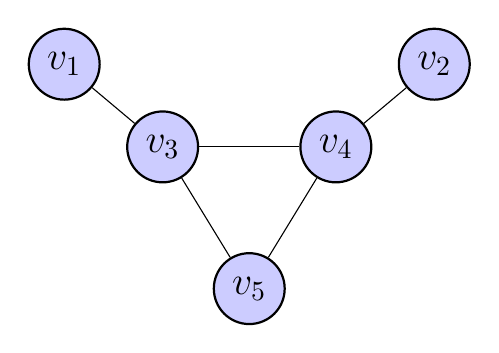
\begin{tikzpicture}[
  scale=1,
  vnode/.style={circle, fill=blue!20, draw=black, thick, minimum size=9mm, inner sep=0pt, font=\Large}
]
  % Vértices
  \node[vnode] (v1) at (0, 3.1) {$v_1$};
  \node[vnode] (v2) at (4.7, 3.1) {$v_2$};
  \node[vnode] (v3) at (1.25, 2.05) {$v_3$};
  \node[vnode] (v4) at (3.45, 2.05) {$v_4$};
  \node[vnode] (v5) at (2.35, 0.25) {$v_5$};

  % Aristas
  \foreach \from/\to in {v1/v3, v2/v4, v3/v4, v3/v5, v4/v5}
    \draw (\from) -- (\to);
\end{tikzpicture}
}}}$
            &
            $\vcenter{\hbox{$\displaystyle \begin{pmatrix}
         0 & 0 & 1 & 0 & 0 \\
         0 & 0 & 0 & 1 & 0 \\
         1 & 0 & 0 & 1 & 1 \\
         0 & 1 & 1 & 0 & 1 \\
         0 & 0 & 1 & 1 & 0
      \end{pmatrix}$}}$ \\
            \noalign{\vspace{6pt}}
         \end{tabular}%
      } \\
      \hline
      \multicolumn{3}{c}{\textbf{Topología de adyacencia}} \\
      \hline
      Abiertos subbásicos & Vecindades mínimas & Topología \\
      \hline
         ${A_{v_1}=\{v_3\}}$\par
         ${A_{v_2}=\{v_4\}}$\par
         ${A_{v_3}=\{v_1,v_4,v_5\}}$\par
         ${A_{v_4}=\{v_2,v_3,v_5\}}$\par
         ${A_{v_5}=\{v_3,v_4\}}$
      &
         ${U_{v_1}=\{v_1,v_4,v_5\}}$\par
         ${U_{v_2}=\{v_2,v_3,v_5\}}$\par
         ${U_{v_3}=\{v_3\}}$\par
         ${U_{v_4}=\{v_4\}}$\par
         ${U_{v_5}=\{v_5\}}$
      &
         $\{\emptyset,$ $\{v_3\},$ $\{v_4\},$ $\{v_5\},$ $\{v_3,v_4\},$ $\{v_3,v_5\},$ $\{v_4,v_5\},$ $\{v_1,v_4,v_5\},$ $\{v_2,v_3,v_5\},$ $\{v_3,v_4,v_5\},$ $\{v_1,v_3,v_4,v_5\},$ $\{v_2,v_3,v_4,v_5\},$ $\{v_1,v_2,v_3,v_4,v_5\}\}$ \\[6pt]
      \hline
      \multicolumn{3}{c}{\textbf{Topología de incidencia}} \\
      \hline
      Abiertos subbásicos & Vecindades mínimas & Topología \\
      \hline
         ${e_{1}=\{v_1,v_3\}}$\par
         ${e_{2}=\{v_2,v_4\}}$\par
         ${e_{3}=\{v_3,v_4\}}$\par
         ${e_{4}=\{v_3,v_5\}}$\par
         ${e_{5}=\{v_4,v_5\}}$
      &
         ${U_{v_1}=\{v_1,v_3\}}$\par
         ${U_{v_2}=\{v_2,v_4\}}$\par
         ${U_{v_3}=\{v_3\}}$\par
         ${U_{v_4}=\{v_4\}}$\par
         ${U_{v_5}=\{v_5\}}$
      &
         $\{\emptyset,$ $\{v_3\},$ $\{v_4\},$ $\{v_5\},$ $\{v_1,v_3\},$ $\{v_2,v_4\},$ $\{v_3,v_4\},$ $\{v_3,v_5\},$ $\{v_4,v_5\},$ $\{v_1,v_3,v_4\},$ $\{v_1,v_3,v_5\},$ $\{v_2,v_3,v_4\},$ $\{v_2,v_4,v_5\},$ $\{v_3,v_4,v_5\},$ $\{v_1,v_2,v_3,v_4\},$ $\{v_1,v_3,v_4,v_5\},$ $\{v_2,v_3,v_4,v_5\},$ $\{v_1,v_2,v_3,v_4,v_5\}\}$ \\[6pt]
      \hline
   \end{tabular}
   \caption{Topologías de adyacencia e incidencia de $G_9$}
   \label{tab:topologias_G_9}

   \vspace{2em}
   \begin{minipage}{\textwidth}
      \normalsize
      El grafo $G_9$ es conocido como \textit{grafo toro}.
   \end{minipage}
\end{table}
